% $Header: /cvsroot/latex-beamer/latex-beamer/doc/beamercolorthemeexample.tex,v 1.11 2004/10/07 20:53:04 tantau Exp $
\documentclass{beamer}

\usepackage{beamerthemesplit}
\usepackage{graphicx,amsmath,natbib} %,apalike,cite
\usepackage{color}
\usepackage{subfigure}
\usepackage{bbm}
\usepackage{mathtools}
\usepackage{enumerate}
\usepackage{framed}
\usepackage{colortbl}
\usepackage{empheq}


%\usepackage{graphicx,times,amsmath}

\DeclarePairedDelimiter\ceil{\lceil}{\rceil}
\DeclarePairedDelimiter\floor{\lfloor}{\rfloor}

\setbeamertemplate{footline}[frame number]

\usetheme{Frankfurt}
\usecolortheme{seahorse}
\usecolortheme{rose}

\newcommand{\bfalpha} {\boldsymbol{\alpha}}
\newcommand{\bfbeta} {\boldsymbol{\beta}}
\newcommand{\bfgamma} {\boldsymbol{\gamma}}
\newcommand{\bfdelta} {\boldsymbol{\delta}}
\newcommand{\bfxi} {\boldsymbol{\xi}}
\newcommand{\bfmu} {\boldsymbol{\mu}}
\newcommand{\bfsigma} {\boldsymbol{\sigma}}
\newcommand{\bfeta} {\boldsymbol{\eta}}
\newcommand{\bfzeta} {\boldsymbol{\zeta}}
\newcommand{\bfvarphi} {\boldsymbol{\varphi}}
\newcommand{\bflambda} {\boldsymbol{\lambda}}
\newcommand{\bfpsi} {\boldsymbol{\psi}}
\newcommand{\bfphi} {\boldsymbol{\phi}}
\newcommand{\bfvarpsi} {\boldsymbol{\varpsi}}
\newcommand{\bfvarsigma} {\boldsymbol{\varsigma}}
\newcommand{\bfnu} {\boldsymbol{\nu}}
\newcommand{\bftheta} {\boldsymbol{\theta}}
\newcommand{\bfomega} {\boldsymbol{\omega}}
\newcommand{\bfTheta} {\boldsymbol{\Theta}}
\newcommand{\bfSigma} {\boldsymbol{\Sigma}}
\newcommand{\bfPsi} {\boldsymbol{\Psi}}
\newcommand{\bfchi} {\boldsymbol{\chi}}
\newcommand{\bfvartheta} {\boldsymbol{\vartheta}}

\newcommand{\bfx} {\mathbf{x}}
\newcommand{\by} {\mathbf{y}} 
\newcommand{\bfy} {\mathbf{y}}
\newcommand{\bfY} {\mathbf{Y}}


\renewcommand{\Pr}{\mathsf{Pr}}
\newcommand{\E}{\mathsf{E}}
\newcommand{\V}{\mathsf{Var}}
\newcommand{\Cov}{\mathsf{Cov}}
\newcommand{\Cor}{\mathsf{Cor}}
\newcommand{\reals}{\mathbb{R}}

\DeclareMathOperator{\diag}{diag}
\DeclareMathOperator{\trace}{tr}
\newcommand{\normal}{\mathsf{N}}
\newcommand{\DP}{\mathsf{DP}}
\newcommand{\Ber}{\mathsf{Ber}}
\newcommand{\Dir}{\mathsf{Dir}}
\newcommand{\Gam}{\mathsf{G}}
\newcommand{\IGam}{\mathsf{IG}}
\newcommand{\bin}{\mathsf{Bin}}
\newcommand{\geo}{\mathsf{Geo}}
\newcommand{\Exp}{\mathsf{E}}
\newcommand{\Wis}{\mathsf{W}}
\newcommand{\IWis}{\mathsf{IW}}
\newcommand{\Poi}{\mathsf{Poi}}
\newcommand{\bet}{\mathsf{beta}}
\newcommand{\Mul}{\mathsf{Mult}}
\newcommand{\GDir}{\mathsf{GDir}}
\newcommand{\nDP}{\mathsf{nDP}}
\newcommand{\HDP}{\mathsf{HDP}}
\newcommand{\NIG}{\mathsf{NIG}}
\newcommand{\PDP}{\mathsf{PDP}}
\newcommand{\CRP}{\mathsf{CRP}}
\newcommand{\SB}{\mathsf{SB}}


\title{Estimation of Volatility Using Open, Close, High, and Low Prices: Application to Stochastic 
Volatility Models and High-Frequency Data.}
\institute{Applied Mathematics and Statistics, \\ University of California, Santa Cruz}
\author{Georgi Dinolov}
\date{September 11, 2014}

\begin{document}

%\frame{\titlepage}

\begin{frame}
  \titlepage
\end{frame}




%\begin{frame}{Motivation}
%
%\begin{tabular}{cc}
%\begin{minipage}{0.5\textwidth}
%	
%\[ \]
%
%\end{minipage}
%&
%\begin{minipage}{0.5\textwidth}
%	\begin{center}
%		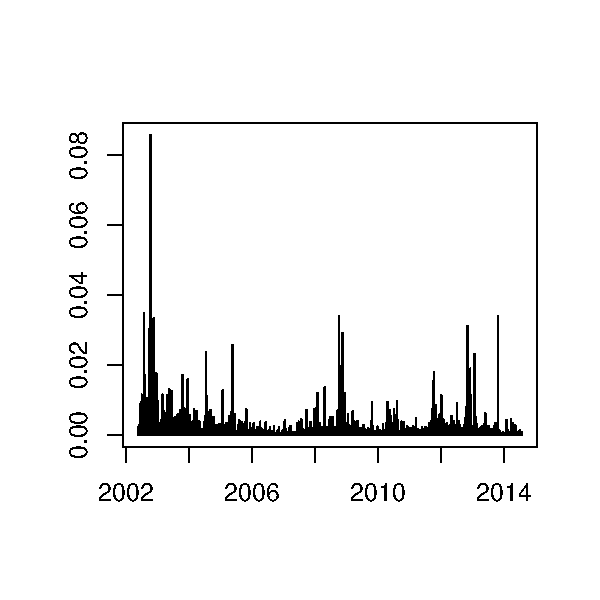
\includegraphics[scale=0.4,angle=0]{./section-1-figures/Netflix-daily-squared-log-returns.pdf}\\
%		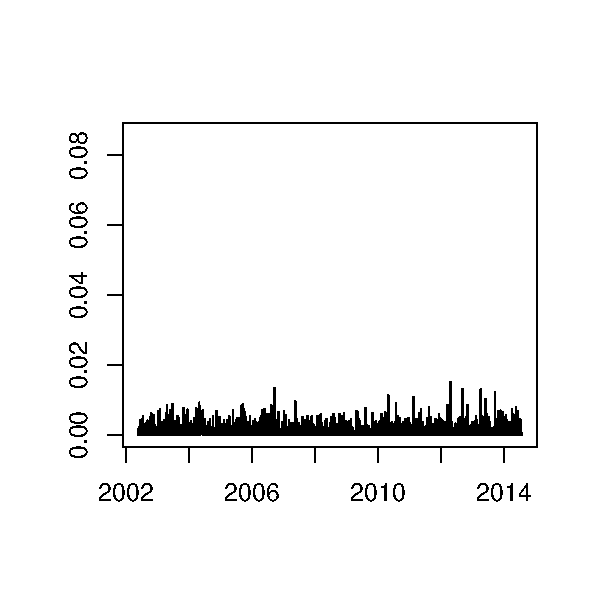
\includegraphics[scale=0.4,angle=0]{./section-1-figures/Netflix-daily-squared-log-returns-constant-vol.pdf}
%	\end{center}
%\end{minipage}
%\end{tabular}
%
%
%
%\begin{centering}
%\textbf{We want to model the change in $\boldsymbol{\sigma}$ over time}
%\end{centering}
%
%\end{frame}





\begin{frame}{Motivation}

\begin{tabular}{cc}
\begin{minipage}{0.5\textwidth}
	\begin{itemize}
		\item Working with returns
		\begin{eqnarray*} 
			\lefteqn{ r_{t+\Delta} \equiv Y_{t + \Delta} - Y_t = } \\
			&&\log(S_{t+\Delta}/S_t) \sim N\left( \Delta \mu, \Delta \sigma^2\right).
		\end{eqnarray*}
		
		\pause	
		\item Log price $Y_t = \log(S_t)$
		\[ d Y_t = \mu dt + \sigma dW_t \]
		
		\pause
		\item Geometric Brownian motion (GBM)
		\[dS_t = \mu S_t dt + S_t \sigma dW_t\]
	\end{itemize}
\end{minipage}
&
\pause
\begin{minipage}{0.5\textwidth}
	\begin{center}
		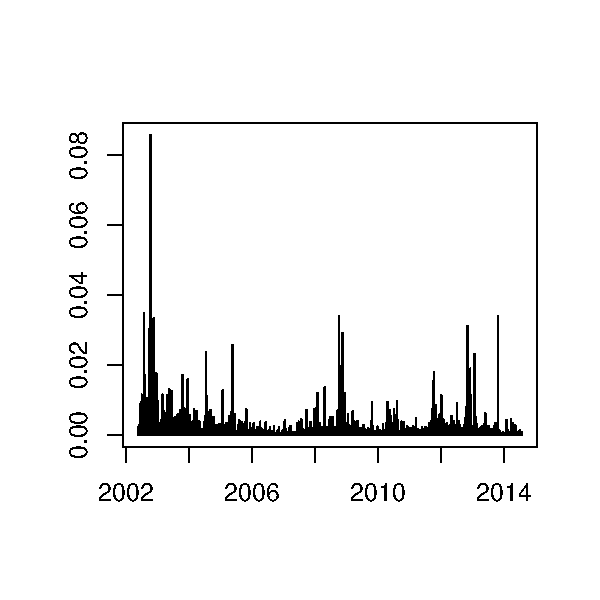
\includegraphics[scale=0.4,angle=0]{./section-1-figures/Netflix-daily-squared-log-returns.pdf}\\
		\vspace{-5mm}
		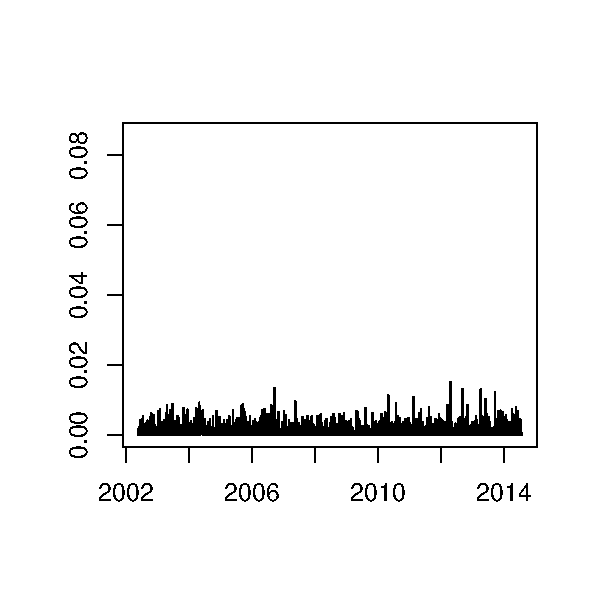
\includegraphics[scale=0.4,angle=0]{./section-1-figures/Netflix-daily-squared-log-returns-constant-vol.pdf}
	\end{center}
\end{minipage}
\end{tabular}

\end{frame}





\begin{frame}{Outline}
  \tableofcontents
\end{frame}

\section{Models for Time-Dependent Volatility}

\begin{frame}{Outline}
  \tableofcontents[currentsection]
\end{frame}

\begin{frame}{Models for Time-Dependent Volatility}
	\begin{enumerate}[1.]
		%\pause
		\item ARCH/GARCH: 
			\begin{align*}
				r_t &= \mu + \epsilon_t & \epsilon_t \sim N(0, \sigma_t^2), \\
				\sigma^2_t &= \omega + \alpha\sigma^2_{t-1} + \beta \epsilon^2_{t-1}	&
			\end{align*}

		%\pause
		\item Time-changed Brownian Motion: BM where the time of the process is scaled 
\[ Y_t = W_{\tau_t}, \,\, t \geq 0; \quad Y_t | \tau_t \sim N(0, \tau_t) \]

		%\pause
		\item Stochastic volatility: 
			\begin{align*}
				Y_t 			&= \mu + Y_{t-1} + \epsilon_t^1 								 & \epsilon_t^1 \sim N(0, \sigma_t^2), \\
				\log(\sigma_t) &= \alpha + \phi \left[ \log(\sigma_{t-1}) - \alpha \right] + \epsilon_t^2  & \epsilon_t^2 \sim N(0, \tau^2)
			\end{align*}
	\end{enumerate}
\end{frame}
	
\begin{frame}{Stochastic Volatility Models}
\begin{itemize}
		\item General case
		\begin{eqnarray*}
			dY_t &=& \mu(Y_t, \sigma_t)dt + \nu(Y_t, \sigma_t)dW_{t,1} \\
			d\sigma_t &=& \alpha(Y_t, \sigma_t)dt + \beta(Y_t, \sigma_t)dW_{t,2}
		\end{eqnarray*}
%
%
		\item Continuous time OU
%
		\begin{eqnarray*}
			d Y_t &=& \mu dt + \sigma_t dW_{t,1} \\
			d \log( \sigma_t ) &=& \underbrace{ \phi(\alpha - \log(\sigma_t))dt + \omega dW_{t,2} }_{\mbox{mean-reverting stochastic process}}
		\end{eqnarray*}
%
		\item Discrete time OU
%		
		\begin{align*}
			Y_t 			&= \mu + Y_{t-1} + \epsilon_t^1 								 & \epsilon_t^1 \sim N(0, \sigma_t^2) \\
			\log(\sigma_t) &= \alpha + \phi \left[ \log(\sigma_{t-1}) - \alpha \right] + \epsilon_t^2  & \epsilon_t^2 \sim N(0, \tau^2)
		\end{align*}
%
	\end{itemize}


\end{frame}



\begin{frame}{High-Frequency Data and Microstructure Noise}
	\begin{itemize}
		%\pause
		\item Availability of tick-by-tick/bid-ask financial transaction data has motivated the development of models that utilize this information to better estimate asset volatility. 
		
		%\pause
		\item A model-free estimation approach: Realized Volatility
				\[ RV^{(m)} = \sum_{i=1}^m r_i^{(m)^2} \]
	It can be shown that $RV^{(m)} \xrightarrow{p} \int_t^{t+\Delta} \sigma^2(Y_s, s)ds$ as $m \to \infty$.

		%\pause
		\item Problem: microstructure noise on the microsecond level
	\end{itemize}
\end{frame}



\section{Univariate Model}
\begin{frame}{Outline}
  \tableofcontents[currentsection]
\end{frame}

\begin{frame}{Motivation}

\begin{itemize}
	\item GARCH/SV models have been adapted to high-frequency data using RV: subsampling and using RV to summarize intraperiod data.

	\item We focus on an approach which collapses high-frequency intraperiod transaction information in the form of recorded maximum and minimum prices.
\end{itemize}
%		 
%\begin{enumerate}[1.]
%	\item \cite{alizadeh2002range} use only the range of the price level
%	\item \cite{lildholdt2002estimation} uses open, close, high, and low (OCHL) data to do maximum likelihood estimation in a GARCH framework
%	\item \cite{rodriguez2012} combine the use of OCHL data with a Bayesian approach to estimation and prediction in a stochastic volatility framework
%\end{enumerate}	
%	
\end{frame}



\begin{frame}{Likelihood for OCHL Data}
\begin{itemize}
	\item We assume constant $\mu$ and $\sigma$ over an interval $s \in [t-1,t]$ with intraperiod min/max $a_t$ and $b_t$,	with BM for the log-price
\begin{eqnarray*}
	dY_s &=& \mu ds + \sigma dW_s, \label{eq:SDE-bc-1} \\
	a_t < &Y_s& < b_t. \label{eq:SDE-bc-2}
\end{eqnarray*}

\pause
	\item Using the Fokker-Planck equation,
\begin{eqnarray*}
	\frac{\partial}{\partial s} q(y,s) &=& -\mu \frac{\partial}{\partial y}q(y,s) + \frac{1}{2}\sigma^2 \frac{\partial^2}{\partial y^2} q(y,s),  \label{eq:IV-BC-1} \\
	q(y,t-1) &=& \delta(y-y_{t-1}); \quad q(a_t,s) = 0, q(b_t, s) = 0 \label{eq:IV-BC-2} \\ 
\end{eqnarray*}
\vspace{-10mm}
%\pause
\[
\boxed{
	q(y,t) = p( m_t \geq a_t, M_t \leq b_t, Y_t = y | Y_{t-1} = y_{t-1})
}
\]
%PDE equivalent to heat equation on bounded domain.
\pause
\vspace{-2mm}
	\item 
Likelihood for OCHL data
\[ 
\boxed{
-\frac{\partial^2 }{\partial a_t \partial b_t } q(y,t) = p( m_t = a_t, M_t = b_t, Y_t = y | Y_{t-1} = y_{t-1})
}
\]
\end{itemize}
\end{frame}



\begin{frame}{Solution by Fourier Expansion}
%Eliminate the advection term through a transformation
%	\begin{equation*}
%		q(y,t) = \exp(ay + bt) \boxed{p(y,t)} \to \frac{\partial}{\partial s} p(y,s) = \frac{1}{2}\sigma^2 \frac{\partial^2}{\partial y^2} p(y,s) 
%	\end{equation*}
%
%\pause
%\begin{tabular}{cc}
%\begin{minipage}{5cm}
%\[ p(y,s) = \sum_{n=1}^\infty C(s)_{n} \sin\left( \frac{n\pi (y- a_t)}{b_t - a_t} \right) \]
%\end{minipage}
%&
%\begin{minipage}{5cm}
%\begin{center}
%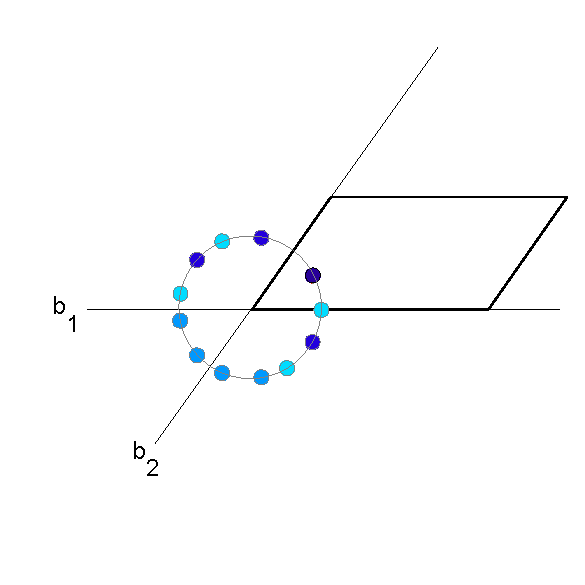
\includegraphics[scale=0.1,angle=0]{./section-3-figures/transformed-reflection.pdf}\\
%\end{center}
%\end{minipage}
%\end{tabular}
%

%\pause
	\begin{eqnarray*}
		\lefteqn{ q(y,t) = \exp\left( \frac{\sqrt{2\mu}}{\sigma} y \right) \times} \\
		&&  \sum_{n=1}^\infty \frac{2}{L} \sin\left( (y_{t-1} - a_t) \frac{n \pi}{L} \right) \exp\left( -\frac{1}{2}\sigma^2 \frac{n^2 \pi^2}{L^2} t \right) \sin\left( (y-a_t) \frac{n\pi}{L} \right) \label{eq:q-final}
	\end{eqnarray*}	

\end{frame}






\begin{frame}{Solution by Method of Images}
\pause

\begin{centering}
\vspace{-15mm}
\begin{tabular}{ccc}
\hspace{-10mm}
\begin{minipage}{0.3\textwidth}
	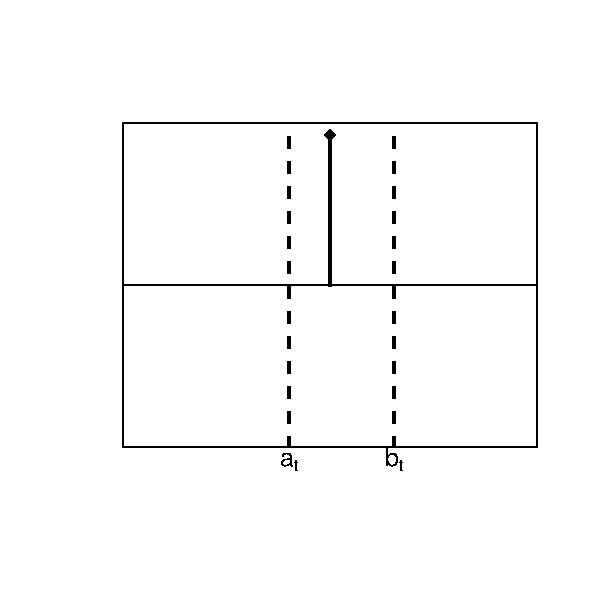
\includegraphics[scale=0.4,angle=0]{./section-2-figures/ic.pdf}
\end{minipage}
\pause

&

\begin{minipage}{0.3\textwidth}
	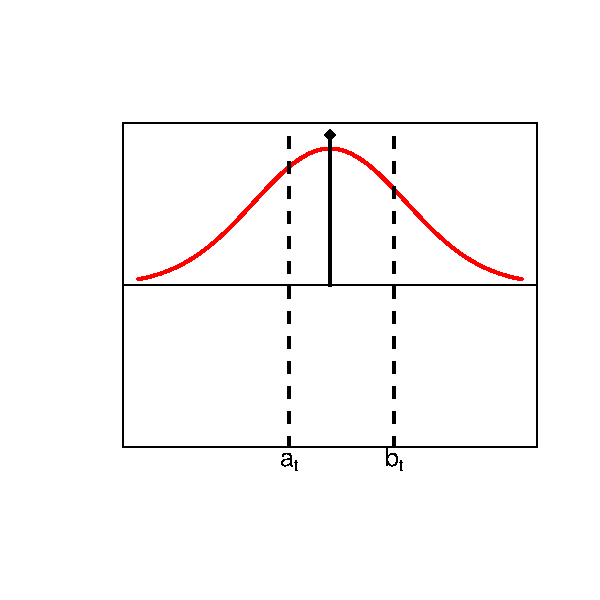
\includegraphics[scale=0.4,angle=0]{./section-2-figures/g0.pdf}
\end{minipage}
\pause

&	

\begin{minipage}{0.3\textwidth}
	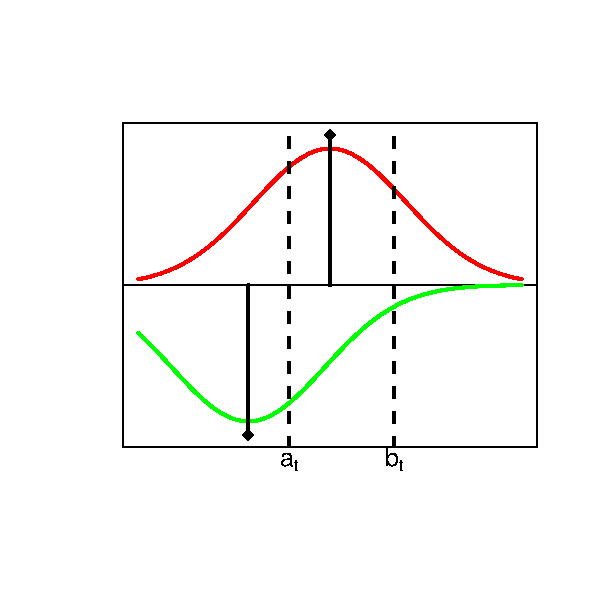
\includegraphics[scale=0.4,angle=0]{./section-2-figures/g0r0.pdf}
\end{minipage}
\vspace{-15mm}
\\\hspace{-10mm}
\pause

\begin{minipage}{0.3\textwidth}
	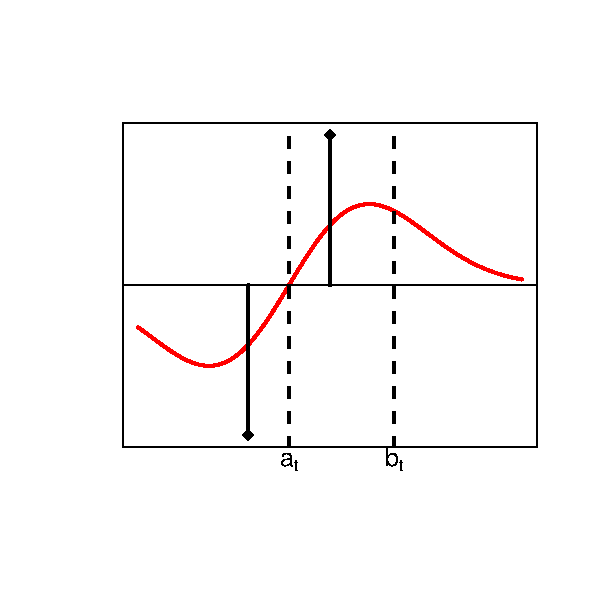
\includegraphics[scale=0.4,angle=0]{./section-2-figures/g1.pdf}
\end{minipage}
\pause

&

\begin{minipage}{0.3\textwidth}
	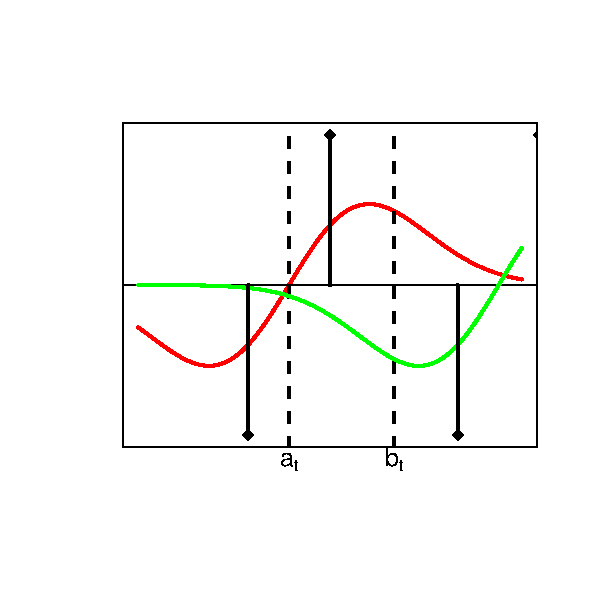
\includegraphics[scale=0.4,angle=0]{./section-2-figures/g1r1.pdf}
\end{minipage}
\pause

&

\begin{minipage}{0.3\textwidth}
	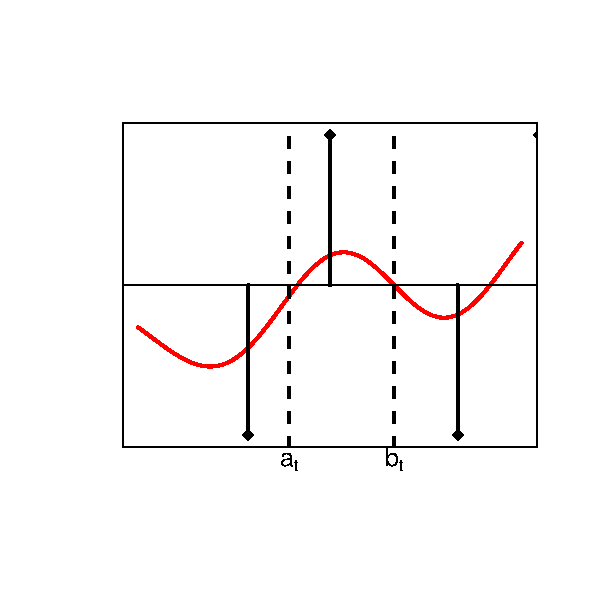
\includegraphics[scale=0.4,angle=0]{./section-2-figures/g2.pdf}
\end{minipage}
\vspace{-15mm}
\\\hspace{-10mm}
\pause

\begin{minipage}{0.3\textwidth}
	\[ \]
\end{minipage}

&

\begin{minipage}{0.3\textwidth}
	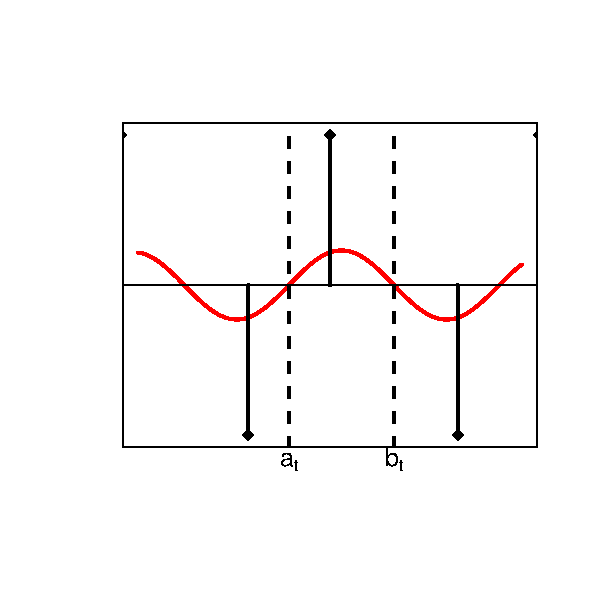
\includegraphics[scale=0.4,angle=0]{./section-2-figures/g3.pdf}
\end{minipage}
\vspace{-20mm}

& 

\begin{minipage}{0.3\textwidth}
	\[ \]
\end{minipage}


\end{tabular}
\end{centering}


\end{frame}


%\begin{frame}{Solution by Method of Images}
%
%\begin{center}
%
%\begin{tabular}{c}
%
%\begin{minipage}{1\textwidth}
%
%\[ q(y,s) = \exp\left( \frac{\sqrt{2\mu}}{\sigma} y \right) \times \]
%\[ \Bigg\{ N( y ; y_{t-1}, s\sigma^2) - N( y ; \zeta(y_{t-1}), s\sigma^2) - N( y ; \xi(y_{t-1}), s\sigma^2) + \]
%\[ \quad \sum_{n=1}^\infty \left[ N( y ; (\xi \circ \zeta)^n (y_{t-1}), s\sigma^2) + N(y ; (\zeta \circ \xi)^n (y_{t-1}), s\sigma^2 ) \right. \]
%\[ \qquad \left. -  N( y ; (\xi \circ \zeta)^n \circ \xi (y_{t-1}), s\sigma^2) - N( y ; (\zeta \circ \xi)^n \circ \zeta (y_{t-1}), s\sigma^2) \right] \Bigg\} \]
%
%\end{minipage}
%
%\end{tabular}
%
%\end{center}
%
%\end{frame}





\begin{frame}{Accuracy of the Fourier Expansion Solution}
\begin{itemize}
	\item Numerical differentiation: central-difference method 
	\[ \Delta x = \frac{1}{2^k} \frac{1}{100} (b_t - a_t). \]
	\item Analytic differentiation
\end{itemize}

\pause
\begin{centering}
\begin{tabular}{|c|c|c|c|c|c|}
\multicolumn{6}{c}{Relative error} \\\hline
		& N=4 & N=8 & N=16 & N=32 & N=64  \\\hline
k=4 &-1.290e-3	&1.810e-5& 1.818e-5 & 1.818e-5 & 1.818e-5 \\\hline
k=8 & -1.308e-3 & 7.110e-8 & 7.111e-8  &	7.111e-8 & 7.111e-8 \\\hline
analytic & -1308e-3	& -2.002e-14&0&	0&	0 \\\hline
\end{tabular}
\end{centering}
(N = number of summands in the truncated expansion; $\mu=1, \sigma=1$, $a_t = -0.0557$, $b_t = 3.1424$, $y_t = 3.019$, $y_{t-1} = 0$. )
\end{frame}



\begin{frame}{Simulation}
	\begin{itemize}
		\item Goal: compare OCHL estimators to RV estimators
		\item Forward-Euler discretization
			\[ Y_{k+1} = Y_{k} + \mu \Delta t^* + \sigma \Delta t^* \epsilon_k \]
		\item $\Delta t^* = 1/23400$, equivalent to sampling the returns once every second over the length of a trading day.
			\[ \mu = 7.936508 \cdot 10^{-5}, \qquad \sigma = 0.01259882 \]	
		\item When performing estimation, longer sampling intervals are used: 5 sec to 7 hours.
		
		\item No microstructure noise
		
		\item 1000 trading days: 1000 estimates for each sampling period $\Delta t$ used. 
	\end{itemize}
\end{frame}




\begin{frame}
	\centering
	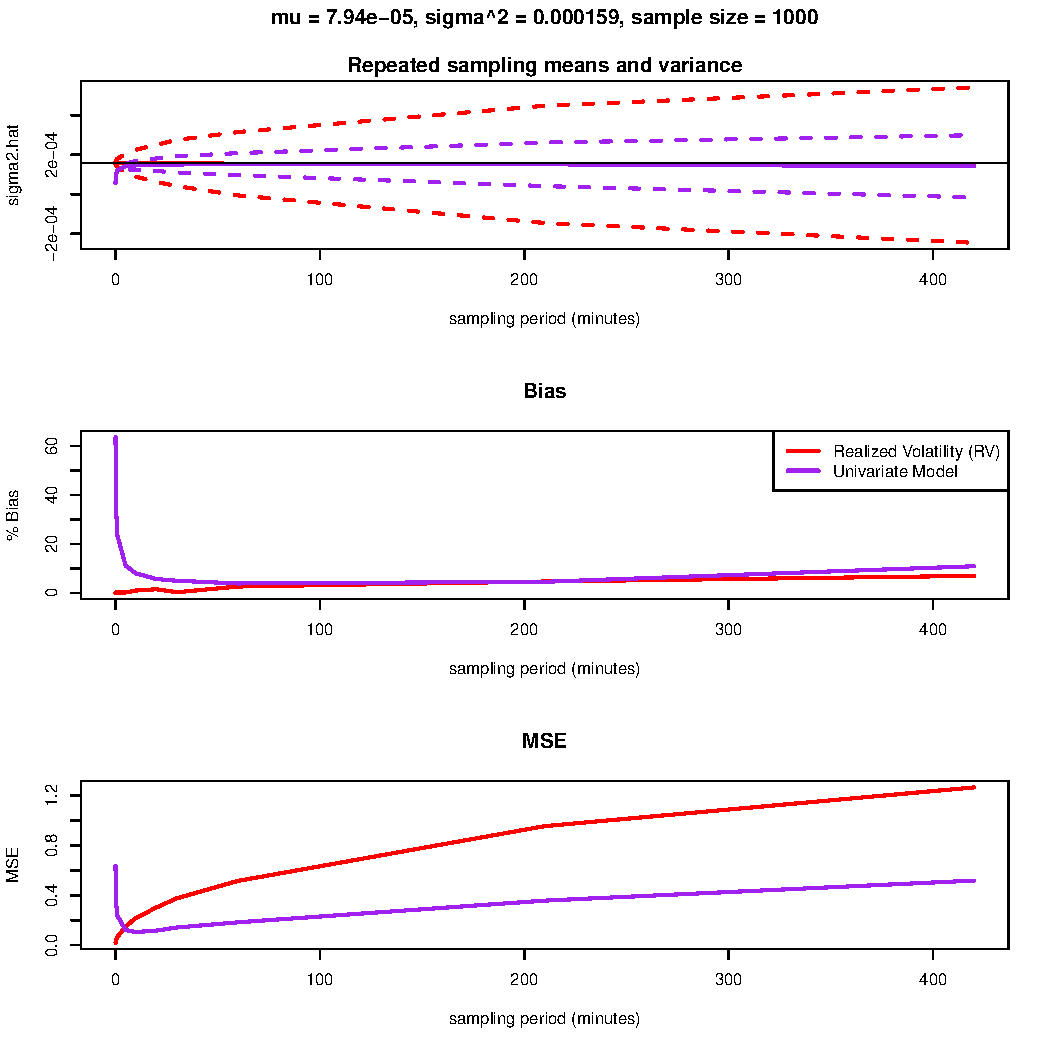
\includegraphics[scale=0.45]{./section-2-figures/results-7-14-13-5-53.pdf}
\end{frame}


\section{Bivariate Model}

\begin{frame}{Outline}
  \tableofcontents[currentsection]
\end{frame}

\begin{frame}{Bivariate Model}
	
	\begin{itemize}
		\item We expect that using OCHL data for two assets can improve estimates for drift and volatility, as well as the estimate of their correlation.

%
\[
	\left. \begin{array}{rcl}
			dY_{1,s} &=& \mu_1 ds + \sigma_1 dW_{1,s}, \\
			dY_{2,s} &=& \mu_2 ds + \sigma_2 dW_{2,s}
		\end{array} \right\} Cor(W_1, W_2) = \rho
\]

\item Through Fokker-Planck equation, with $\mathbf{y} = (y_1, y_2)$,

\begin{equation*}
	\frac{\partial}{\partial s} q(\by, s) = -\mu_1 \frac{\partial}{\partial y_1}q(\by,s) -\mu_1 \frac{\partial}{\partial y_2}q(\by,s)
\end{equation*}
\[ + \frac{1}{2}\sigma_1^2 \frac{\partial^2}{\partial y_1^2} q(\by,s) + \frac{1}{2} \sigma_2^2 \frac{\partial^2}{\partial^2 y_2}q(\by,s) + \rho \sigma_1 \sigma_2 \frac{\partial^2}{\partial y_1 \partial y_2} q(\by, s) \]
\begin{eqnarray*}
	q(\by, t-1) &=& \delta(y_1-y_{1,t-1})\delta(y_2-y_{2,t-1}), \label{eq:ch3-IC-BV-2} \\
	q(\by, s) &=& 0 \quad \mbox{for} \quad y_1 = a_{1,t}, b_{1,t} \,\, \mbox{ or } \,\, y_2 = a_{2,t}, b_{2,t}. \label{eq:ch3-IC-BV-3}
\end{eqnarray*}

\end{itemize}
\end{frame}



\begin{frame}{Solution through Method of Images}
 
{\color{red} Method of Images does not work.}
\vspace{10mm}
%\[
%\frac{\partial p(\boldsymbol{\zeta},s)}{\partial s} = \frac{1}{2}\tilde{\sigma}_1^2 \frac{\partial^2}{\partial \zeta_1^2} p(\boldsymbol{\zeta},s) + \frac{1}{2} \tilde{\sigma}_2^2 \frac{\partial^2}{\partial^2 \zeta_2}p(\boldsymbol{\zeta},s).
%\]

\begin{tabular}{cc}
\begin{minipage}{5cm}
\begin{center}
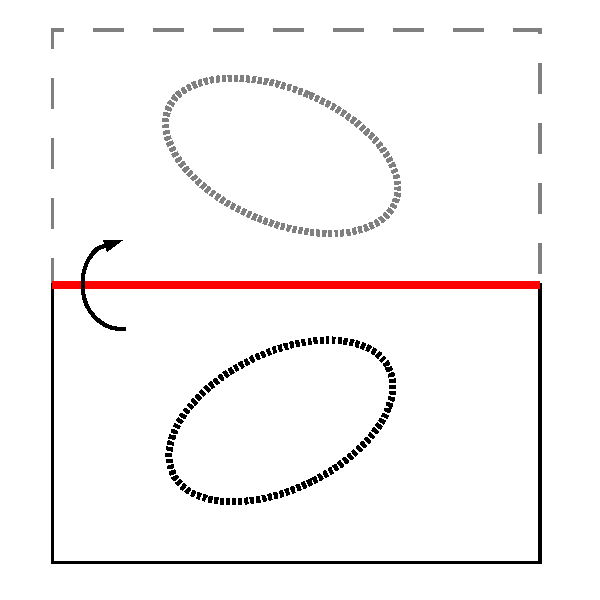
\includegraphics[scale=0.5,angle=0]{./section-3-figures/unmodified-reflection.pdf}
\end{center}
\end{minipage}
&
\begin{minipage}{5cm}
\begin{center}
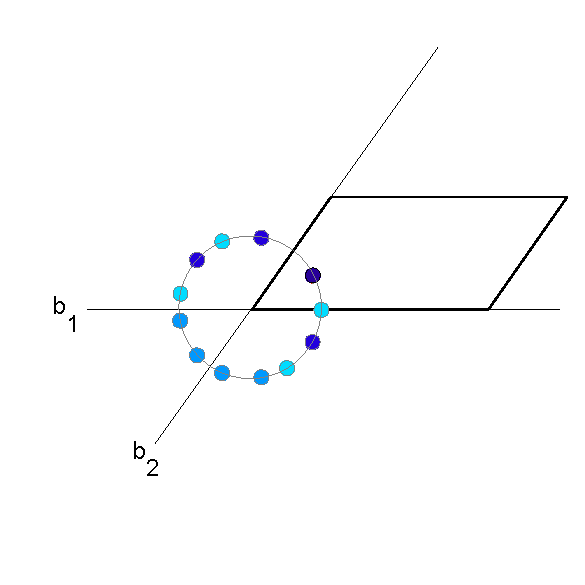
\includegraphics[scale=0.6,angle=0]{./section-3-figures/transformed-reflection.pdf}\\
\end{center}
\end{minipage}
\end{tabular}

\end{frame}



\begin{frame}{Solution through Fourier Expansion}
\begin{eqnarray*}
\lefteqn{	q(\mathbf{y}, s) = \exp(\mathbf{a}^T \by + bs) \times } \\
	&& \sum_{m=1}^\infty \sum_{n=1}^\infty C_{m,n}(s) \sin\left( \frac{m \pi (y_1 - a_{1,t})}{b_{1,t} - a_{1,t}} \right) \sin\left( \frac{n \pi (y_2 - a_{2,t})}{b_{2,t} - a_{2,t}} \right) \\
	&&= \exp(\mathbf{a}^T \by + bs) \left(  \mathbf{C}(s)^T \mathbf{S} \right)
\end{eqnarray*}

\begin{equation*}
	\frac{d}{ds} \left( \begin{array}{c} 
			C_{1,1}(s) \\
				\vdots \\
			C_{1,N}(s) \\
			C_{2,1}(s) \\
				\vdots \\
			C_{M,N}(s)
		\end{array} \right) = \underbrace{ \frac{1}{2}\sigma^2_1 \mathbf{A}_1 + \frac{1}{2}\sigma^2_2 \mathbf{A}_2 + \rho\sigma_1 \sigma_2 \mathbf{B} }_{\mathbf{A}} \left( \begin{array}{c} 
			C_{1,1}(s) \\
				\vdots \\
			C_{1,N}(s) \\
			C_{2,1}(s) \\
				\vdots \\
			C_{M,N}(s)
		\end{array} \right) \label{eq:matrix-representation}
\end{equation*}
\end{frame}



\begin{frame}{Evaluating the Likelihood}
	
\[ \frac{\partial^4 q(\by, t)}{\partial a_{1,t}\partial b_{1,t} \partial a_{2,t} \partial b_{2,t} } = \]
		\[p( m_{1,t} = a_{1,t}, M_{1,t} = b_{1,t}, m_{2,t} = a_{2,t}, M_{2,t} = b_{2,t}, \bfY_t = \by | \bfY_{t-1} = \by_{t-1}) \]

\pause	
\begin{itemize}
	\item Numerical differentiation 
		\[ \frac{\partial^4 q(\by, t)}{\partial a_{1,t}\partial b_{1,t} \partial a_{2,t} \partial b_{2,t} } \approx \frac{\mbox{finite difference} + \epsilon_{\mbox{machine}}}{ (\Delta x)^4 }  \]
	
	\pause
	\item Mixed differentiation
\[
	\frac{\partial^4 q(\by, t)}{\partial a_{1,t}\partial b_{1,t} \partial a_{2,t} \partial b_{2,t} } = \exp(\mathbf{a}^T \by + bs)\frac{\partial^4 (  \overbrace{ \boxed{ e^{\mathbf{A}s}\mathbf{C}(0) }^T }^{\mathbf{C}(s)^T} \mathbf{S} )}{\partial a_{1,t}\partial b_{1,t} \partial a_{2,t} \partial b_{2,t} }
\]
\end{itemize}

\end{frame}




\begin{frame}{Numerical Results}

\begin{itemize}
	\item $\Delta x = \min\left\{ \frac{1}{2^k} \frac{1}{100} (b_{1,t} - a_{1,t}), \frac{1}{2^k} \frac{1}{100} (b_{2,t} - a_{2,t}) \right\}$

	\item $N = M$ in Fourier expansion
	\item $\mu_1 = \mu_2 = 1$, $\sigma_1 = \sigma_2 = 1$. 
\end{itemize}

\pause
\begin{centering}
\begin{tabular}{|c|c|c|c|c|c|}
\multicolumn{6}{c}{Log-likelihood for $\rho = 0.3$} \\\hline
		& N=4 & N=8 & N=16 & N=32 & N=64  \\\hline
k=3 &-1.8300 & -1.7475 & -1.7601 & -1.7416 & -1.6371 \\\hline
k=6 & -1.8300 & -1.7475 & -1.7601 & -1.7421 & -1.6453 \\\hline
k=8 & -1.8564 & -1.7292 & -1.8217 & -1.4718 & \cellcolor{red!50}{$-\infty$} \\\hline \hline
mixed, k=3 & -1.8300 & -1.7475 & -1.7601 & -1.7416 & -1.6371 \\\hline
mixed, k=6 & -1.8300 & -1.7475 & -1.7601 & -1.7421 & -1.6453 \\\hline
mixed, k=8 & \cellcolor{blue!50}{-1.8300} & \cellcolor{blue!40}{-1.7475} & \cellcolor{blue!30}{-1.7601}	& \cellcolor{blue!20}{-1.7416} & \cellcolor{blue!10}{-1.6365} \\\hline
\end{tabular}
\end{centering}

\vspace{1mm}
($a_{1,t} = -0.7906$, $b_{1,t} = 0.7947$, $y_{1,t} = -0.3946$, $a_{2,t}=-0.02775$, $b_{2,t} = 1.2675$, $y_{2,t} = 1.06421$)

\end{frame}





\begin{frame}{Numerical Results}

\begin{centering}
\begin{tabular}{|c|c|c|c|c|c|}
\multicolumn{6}{c}{Log-likelihood for $\rho = 0.5$} \\\hline
		& N=4 & N=8 & N=16 & N=32 & N=64  \\\hline
k=3 &--3.3405 & -3.4384 & -3.8774 & -3.9335 & -3.8991 \\\hline
k=6 & -3.3409 & -3.4354 & -3.9105 & -3.9596 & -3.7720 \\\hline
k=8 & -3.3811 & -2.9068 & -5.4378 & \cellcolor{red!50}{$-\infty$} & 1.0481 \\\hline \hline
mixed, k=3 & -3.3405 & -3.4384 & -3.8776 & -3.9338 & -3.8981 \\\hline
mixed, k=6 & -3.3405 & -3.4384 & -3.8778 & -3.9337 & -3.8980 \\\hline
mixed, k=8 & \cellcolor{blue!50}{-3.3405} & \cellcolor{blue!40}{-3.4384} & \cellcolor{blue!30}{-3.8778} & \cellcolor{blue!20}{-3.9337} & \cellcolor{blue!10}{-3.8980} \\\hline
\end{tabular}
\end{centering}

\vspace{1mm}
($b_{1,t} = 0.5524$, $a_{1,t}=-0.7481$, $y_{1,t}=-0.3282$, $b_{2,t}=0.01645$, $a_{2,t}=-2.7176$, $y_{2,t}=-2.1075$
)

\end{frame}




\begin{frame}{Numerical Results}

\begin{centering}
\begin{tabular}{|c|c|c|c|c|c|}
\multicolumn{6}{c}{Log-likelihood for $\rho = 0$} \\\hline
		& N=4 & N=8 & N=16 & N=32 & N=64  \\\hline
k=8 & -2.1731 & -2.1731 & -2.1731 & -2.1731 & -2.1731 \\\hline \hline
mixed, k=8 & -2.1731 & -2.1731 & -2.1731 & -2.1731 & -2.1731 \\\hline
\end{tabular}
\end{centering}

\vspace{1mm}
($b_{1,t}=1.5059$, $a_{1,t}=-0.1894$, $y_{1,t}=1.4004$, $b_{2,t}=0.5387$, $a_{2,t}=-0.2317$, $y_{2,t}=0.2569$)
\end{frame}





\section{Future Work}

\begin{frame}{Outline}
  \tableofcontents[currentsection]
\end{frame}




\begin{frame}{Bernstein Polynomials}
\begin{itemize}
	\item Sparser matrix
	\vspace{-10mm}
	\begin{centering}
	\begin{tabular}{cc}
		\begin{minipage}{0.5\textwidth}
		\[ B_{\nu,n}(x) = \left( \begin{array}{c} n \\ \nu \end{array} \right) x^\nu (1-x)^{n-\nu},\]
		\[\nu = 0, \ldots, n \]
		\end{minipage}
		&
		\begin{minipage}{0.5\textwidth}
			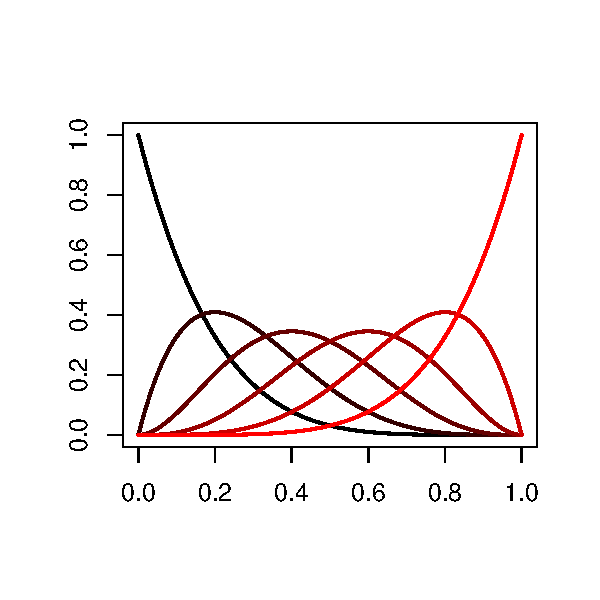
\includegraphics[scale=.5]{./section-4-figures/bernstein.pdf}
		\end{minipage}
	\end{tabular}
	\end{centering}
	\vspace{-10mm}
	\[ q(\by, s) = \sum_{n=1}^N \sum_{m=1}^M C_{m,n}(s) B_{n,N}(y_1) B_{m,M}(y_2). \]

	\item Accounting for correlation 
		\[ q(\by, s) = \sum_{n=1}^N \sum_{m=1}^M C_{m,n}(s) \mathcal{K}\bigg(B_{n,N}(y_1) , B_{m,M}(y_2) \bigg). \]

	\item Other bases?
\end{itemize}

\end{frame}



\begin{frame}{Bivariate Stochastic Volatility Model Using OCHL data}
		\[ \left( \begin{array}{c} \log(S_{t+1,1}) \\ \log( S_{t+1,2}) \end{array} \right) = \left( \begin{array}{c} \log(S_{t,1}) \\ \log( S_{t,2}) \end{array} \right) + \left( \begin{array}{c} \mu_1 \\ \mu_2 \end{array} \right) + \mathbf{V_{t+1}} \left( \begin{array}{c} w_{t+1,1} \\ w_{t+1,2} \end{array} \right) \]

%\pause
\[
 	\mathbf{V}_{t} = \left( \begin{array}{cc} 
					V_{t,11} & 0 \\
					V_{t,21} & V_{t,22}
					\end{array} \right), \qquad \boldsymbol{\Sigma}_t = \mathbf{V}'_{t} \mathbf{V}_t.
\]

%\pause
\[
	\left( \begin{array}{c} \log(V_{t+1,11}) \\ \log(V_{t+1,22}) \\ V_{t+1,21} \end{array} \right) = \left( \begin{array}{c} \mu_{11} \\ \mu_{22} \\ \mu_{21} \end{array} \right) + \boldsymbol{\Psi} \left( \left( \begin{array}{c} \log(V_{t,11}) \\ \log(V_{t,22}) \\ V_{t,21} \end{array} \right) - \left( \begin{array}{c} \mu_{11} \\ \mu_{22} \\ \mu_{21} \end{array} \right) \right) + \boldsymbol{\nu},
\]
\[ \qquad \boldsymbol{\nu} \sim N_3(\mathbf{0}, \boldsymbol{\Sigma}_\nu) \]

\end{frame}




\begin{frame}{Stochastic Volatility Estimation with Microstructure Noise}
%\begin{eqnarray*}
%	Y_{t+1} &=& \log(S_{t+1}) + \xi\gamma_{t} \\	
%	\log(S_{t+1}) &=& \log(S_{t}) + \mu + \sigma_{t+1} \epsilon_{t+1,1} \\
%	\log(\sigma_{t+1}) &=& \alpha + \phi[ \log(\sigma_{t}) - \alpha] + \beta\epsilon_{t+2,2}.
%\end{eqnarray*}

 \[ \hspace{-15mm} Y_{t+1} = \log(S_{t+1}) + \xi\gamma_{t} \]
\begin{subequations}
\begin{empheq}[box=\fbox]{align*}
  \log(S_{t+1}) &= \log(S_{t}) + \mu + \sigma_{t+1} \epsilon_{t+1,1} \\
  \log(\sigma_{t+1}) &= \alpha + \phi[ \log(\sigma_{t}) - \alpha] + \beta\epsilon_{t+2,2}.
\end{empheq}
\end{subequations}
%\pause
\begin{itemize}
	\item $\gamma_t \sim N(0, 1)$, $\xi \approx D/2Q$. 
	\item $(\epsilon_{t+1,1}, \epsilon_{t+1,2})$ follows a bivariate normal distribution with $E(\epsilon_{t,1}) = E(\epsilon_{t,2}) = 0$, $\mbox{Var}(\epsilon_{t,1}) = \mbox{Var}(\epsilon_{t,2}) = 1$ and $\mbox{Cor}(\epsilon_{t,1}, \epsilon_{t,2}) = \rho$. 
	%\item By allowing a nonzero correlation between these innovations, the model incorporates possible leverage effects.
\end{itemize}
\end{frame}




\begin{frame}{Univariate Likelihood in the Presence of Microstructure Noise}
	\begin{itemize}
		\item Our goal is to derive the likelihood for the open, close, high, and low \textbf{observed} prices within a period.
		\item \textbf{Observed} intraperiod maximum and minimum are not the \textbf{true} maximum and minimum taken on by the asset. 

		\item Previous work is not directly applicable in this setting.
		\item Brownian motion with jumps?
	\end{itemize}
\end{frame}





\begin{frame}{Timeline for Future Work}

\begin{minipage}{1\textwidth}
\begin{centering}
\hspace{-4mm}
\scalebox{0.5}{
\begin{tabular}{|l|l|l|l|l|l|l|}\hline
    & Fall 2014 & Winter 2015 & Spring 2015 & Summer 2015 & Fall 2015 & Winter 2016 \\\hline
    {\bf Stochastic Volatility with microstructure noise}: &\cellcolor{cyan} &&&&&\\\hline
    {\bf Univariate Likelihood with microstructure noise}: &\multicolumn{2}{|c|}{\cellcolor{red}} &&&&\\\hline
    {\bf Bivariate Likelihood with Bernstein polynomials}: &&\multicolumn{2}{|c|}{\cellcolor{green}} &&&\\\hline
    {\bf Bivariate Stochastic Volatility model}: &&&\multicolumn{3}{|c|}{\cellcolor{yellow}} &\\\hline
%    {\bf Robotic test bed}: & \multicolumn{6}{|c|}{\cellcolor{brown}}&&\\\hline
    {\bf Thesis writing}: &&&&&\multicolumn{2}{|c|}{\cellcolor{magenta}} \\\hline
\end{tabular}}	
\end{centering}
\end{minipage}

\end{frame}





\begin{frame}{Questions}

\end{frame}





\begin{frame}{Microstructure Variance Specification}
\begin{itemize}
	\item Observe price $P_t$ is the true price $S_t$ plus noise
\[ P_t = S_t + \xi^* \epsilon_t, \quad \xi^* = D/2  \]

	\item The log of the observed price is approximated with a first-order Taylor expansion and with average price $Q$
\begin{eqnarray*}
	\log(P_t) &=& \log(S_t + \xi^* \epsilon_t) \\
		 &\approx& \log(S_t) + \frac{\xi^*}{S_t}\epsilon_t \\
		 &\approx& \log(S_t) + \frac{\xi^*}{Q}\epsilon_t
\end{eqnarray*}

	\item Hence, the standard deviation in the SV model is approximated with 
	\[ \boxed{\xi = D/2Q} \]
\end{itemize}

\end{frame}




\begin{frame}{Analytic Matrix Derivatives}
\begin{itemize}
	%\item $\mathbf{H} = \mathbf{V} \boldsymbol{\Lambda} \mathbf{V}^{-1}$
	\item ``Matrix'' Cauchy	Integral
\[ f(H) = \frac{1}{2\pi i} \oint f(z) (\mathbf{I}z - \mathbf{H})^{-1} dz \]

	\item Differentiation with respect to some parameter $\mu$ 
	\[ \frac{\partial}{\partial \mu}f(H) = \frac{1}{2\pi i} \oint f(z) (\mathbf{I}z - \mathbf{H})^{-1} \frac{\partial \mathbf{H}}{\partial \mu} (\mathbf{I}z - \mathbf{H})^{-1} dz \]

	\item Second-order derivative follow
	\[ \frac{\partial^2}{\partial \mu \partial \nu}f(H) = \] 
	\[\frac{1}{2\pi i} \oint f(z) \frac{\partial}{\partial \nu} \left[ (\mathbf{I}z - \mathbf{H})^{-1} \frac{\partial \mathbf{H}}{\partial \mu} (\mathbf{I}z - \mathbf{H})^{-1} \right] dz  \]
\end{itemize}
\end{frame}





\end{document}

